\def\lim{10}

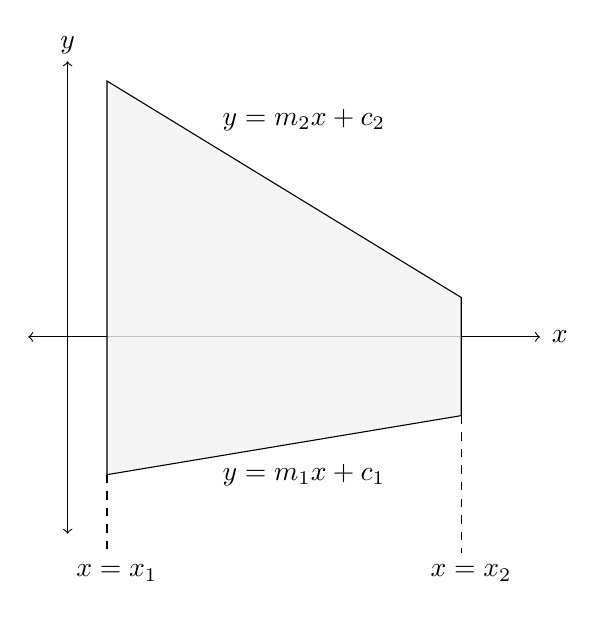
\begin{tikzpicture}[scale=0.5]
	\coordinate(negx) at (-1,0);
	\coordinate(posx) at (\lim+2,0);
	\coordinate(negy) at (0,-5);
	\coordinate(posy) at (0,7);
	
	\coordinate(TL) at (1,6.5);
	\coordinate(BL) at (1,-3.5);
	\coordinate(TR) at (\lim,1);
	\coordinate(BR) at (\lim,-2);
	
	\draw[<->] (negx) -- (posx);
	\draw[<->] (negy) -- (posy);
	\filldraw[fill=black!5, fill opacity=0.8] (BL) -- (BR) -- (TR) -- (TL) -- cycle;
	
	\draw[dashed] (BL) -- (1,-5.5);
	\node(x1) at (1.25,-6) {\(x = x_1\)};
	\draw[dashed] (BR) -- (\lim,-5.5);
	\node(x2) at (\lim+0.25,-6) {\(x = x_2\)};
	\node(m1c1) at (6,-3.5) {\(y=m_1x+c_1\)};
	\node(m2c2) at (6,5.5) {\(y=m_2x+c_2\)};
	\node(x) at (\lim+2.5,0) {\(x\)};
	\node(y) at (0,7.4) {\(y\)};
\end{tikzpicture}